section{Zielsetzung}
Im vorliegenden Experiment wurde zunächst die Spannungskurve eines Selektivverstärkers gemessen. Anschließend wurde mithilfe einer Brückenschaltung paramagnetische Suszeptibilität zweier seltener Erden gemessen.
\section{Theorie}
\subsection{Theoretische Berechnung der paramagnetischen Suszeptibilität}
In Materie wird die Magnetische Flussdichte $\vec{B}=\mu \vec{H}$ um die sogenannte magnetisierung $M$ ergänzt
\begin{equation*}
\vec{B}=\mu _0 \vec{H}+\vec{M}
\end{equation*}
mit der magnetischen Feldstärke $\vec{H}$ und der Induktionskonstante $\mu_0$. Diese entsteht durch atomare magnetische Momente in der Materie
\begin{equation}
\vec{M}=\mu_0N\bar{\vec{\mu}}=\mu_0\chi\vec{H}
\end{equation}
und kann daher einerseits durch das mittlere magnetische Moment $\bar{\vec{\mu}}$ und die Zahl der Momente pro Volumeneinheit $N$ beschrieben werden. Andererseits hängt die Magnetisierung über die Suszeptibilität $\chi$ mit der Feldstärke zusammen.\\ Bei diamagnetischen Stoffen richten sich die magnetischen Momente entgegen des äußeren magnetischen Feldes aus, weshalb sie eine negative Suszeptibilität aufweisen. Der in diesem Versuch untersuchte Paramagnetismus tritt nur bei Substanzen mit nicht verschwindendem Drehimpuls auf und ist im Gegensatz zum Diamagnetismus temperaturabhängig. \\
Der atomare Gesamtdrehimpuls $\vec{L}$ setzt sich aus dem Eigendrehimpuls bzw. dem Spin $\vec{S}$, dem Drehimpuls der Elektronenhülle $\vec{J}$ und dem Kerndrehimpuls zusammen, wobei letzterer jedoch vernachlässigt werden kann. Die verbleibenden Anteile hängen über die sogenannte LS-Kopplung
\begin{equation}
\vec{J}=\vec{L}+\vec{S}
\end{equation}
zusammen. Die zu den Komponenten gehörenden magnetischen Momente ergeben sich aus der Quantenmechanik zu
\begin{equation*}
\vec{\mu_L}=-\frac{\mu_B}{\hbar}\vec{L} 
\end{equation*}
und
\begin{equation*}
\vec{\mu_S}=-g_S\frac{\mu_B}{\hbar}\vec{S}
\end{equation*}
mit dem Bohrschen Magneton $\mu_B$ und dem gyromagnetischen Verhältnis $g_S$. Aus der Beziehung $\lvert \vec{L} \rvert=\sqrt{J(J+1)}\hbar$ (mit der Gesamtdrehimpulsquantenzahl J), die analog mit entsprechenden Quantenzahlen für die anderen Komponenten gilt, lässt sich für die Beträge der betreffenden Momente herleiten:
\begin{equation*}
\lvert \vec{\mu_L}\rvert=\mu_B\sqrt{L(L+1)}
\end{equation*}
bzw.
\begin{equation*}
\lvert \vec{\mu_S}\rvert=g_S\mu_B\sqrt{S(S+1)}
\end{equation*}
\begin{figure}[h]
    \centering
    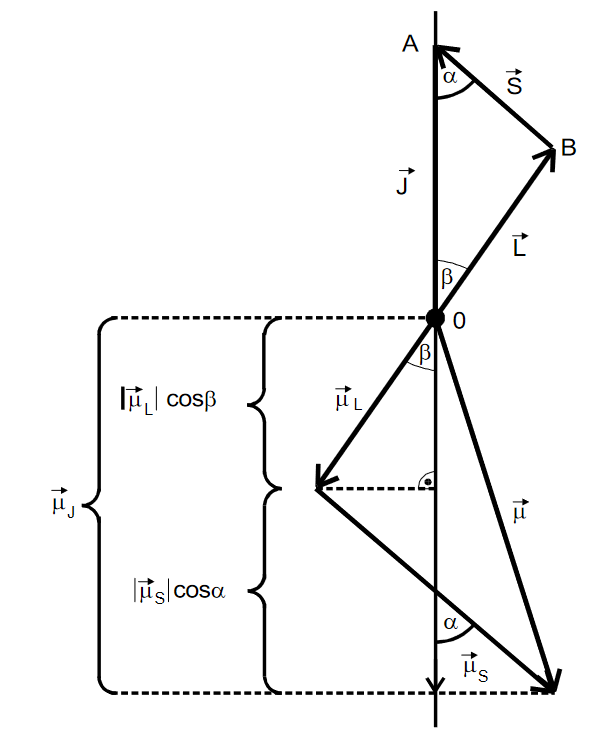
\includegraphics[width=4cm, keepaspectratio]{Drehimpuls}
    \label{Drehimpuls}
  \end{figure}
Unter der Bedingung, dass nur die zu $\vec{J}$ parallele Komponente von $\mu$ messbar ist, lässt sich aus den in der Abbildung gezeigten geometrischen Beziehungen sowie sowie durch den Kosinussatz die Formel
\begin{equation*}
\lvert \vec{\mu_J} \rvert=\mu_B\sqrt{J(J+1)}\frac{3J(J+1)+(S(S+1)-L(L+1))}{2J(J+1)}
\end{equation*}
herleiten. Wobei das gyromagnetische Verhältnis als $g_S\approx2$ genähert wurde. Der Ausdruck
\begin{equation}
g_J\coloneq\frac{3J(J+1)+(S(S+1)-L(L+1)}{2J(J+1)}
\end{equation}
wird als Lande-Faktor bezeichnet. Dadurch vereinfacht sich Gleichung zu
\begin{equation}
\lvert \vec{\mu_J} \rvert=\mu_Bg_J\sqrt{J(J+1)}
\end{equation}
Im Zuge der Quantenmechanik zeigt sich das Phänomen der sogenannten Richtungsquantelung, welche aussagt, dass die Komponente $\mu_Jz$ von$\mu_J$ nur in ganzahligen vielfachen von $\mu_Bg_J$ vorkommen kann, also gilt
\begin{equation*}
\mu_Jz=\mu_Bg_Jm
\end{equation*}
mit der Orientierungsquantenzahl m. Daraus folgt, dass $2J+1$ Orientierungen mit entsprechenden Energieniveaus existieren. \\ 
Mithilfe der sogenannten Bolzman-Verteilung lässt sich nun das mittlere Magnetische Moment berechnen indem die Summe aller möglichen Orientierungen mit zugehöriger Wahrscheinlichkeit durch die Gesamtwahrscheinlichkeit dividiert wird. Dies liefert nach Anwendung der Hochtemparaturnäherung die Formel 
\begin{equation}
\chi=\frac{\mu_0\mu_B^2g_J^2NJ(J+1)}{3kT}
\end{equation}
für die paramagnetische Suszeptibilität. Hier stellt $T$ die Temparatur und $k$ die Bolzman-Konstante dar.
\subsection{Hundsche Regeln}
Bei seltenen Erd Verbindungen sind vornehmlich die Elektronen der 4f-Schale für den Paramagnetiskus verantwortlich. Die Anordnung dieser Elektronen und der von ihnen gebildete Gesamtdrehimpuls wird durch die sogenannten Hundschen Regeln beschrieben:
\begin{itemize}
\item Die einzelnen Spins der Elektronen $s_i$ setzen sich zum maximalen nach dem Pauli-Prinzip möglichen Gesamtspin zusammen
\item Der Gesamtdrehimpuls $\vec{L}$ entspricht der größten unter Regel 1 und dem Pauli-Prinzip möglichen Summe der einzelnen Drehimpulse
\item Wenn die Schale weniger als halb gefüllt ist berechnet sich der Bahndrehimpuls aus $\vec{J}=\vec{L}-\vec{S}$, wenn sie mehr als Halb gefüllt ist aus $\vec{J}=\vec{L}+\vec{S}$
\end{itemize}
\subsection{Messverfahren}
Für die Messung wird der Effekt genutzt, dass sich die Induktivität $L$ einer Spule der Länge $l$ und Windungszahl $n$ durch Einsetzen einer paramagnetischen Probe mit Querschnitt $Q$ um die Differenz
\begin{equation*}
\Delta L=\mu_0 \chi Q \frac{n^2}{l}
\end{equation*}
ändert. 
\begin{figure}[h]
    \centering
    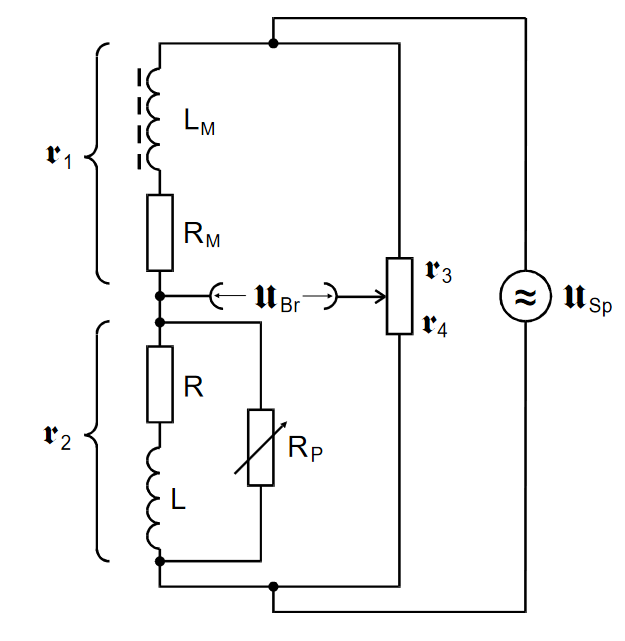
\includegraphics[width=4cm, keepaspectratio]{Brückenschaltung}
    \label{Brückenschaltung}
  \end{figure}
Die Messung der Paramagnetischen Suszeptibilität erfolgt nun mithilfe einer Brückenschaltung, deren Schematischer Aufbau in Abbildung (2) zu sehen ist. Zunächst wird durch Einstellung des Widerstandes die Schaltung  abgeglichen, sodass keine Brückenspannung mehr zu messen ist. Anschließend wird eine Probe in die Spule eingeführt, was zum Auftreten einer Brückenspannung $U_Br$ führt aus welcher sich die Suszeptibilität berechnen lässt. Bei fester Speisespannung $U_Sp$ und Spulenflächenquerschnitt $F$ lässt sie sich durch
\begin{equation}
\chi=4\frac{FU_Br}{QU_Sp}
\end{equation}
berechnen. Nach dem Messen der Brückenspannung muss die Schaltung erneut abgeglichen werden indem der Widerstand $R_3$ um den Wert $\Delta R$ geändert wird. Aus der Widerstandsdifferenz lässt sich erneut die Suszeptibilität berechenen:
\begin{equation}
\chi=2\frac{\Delta R F}{R_3 Q}
\end{equation}
\subsection{Selektivverstärker}
Im Zuge der Messung tritt in an der Brückenschaltung eine Störspannung auf, welche bisweilen sogar groß genug sein kann um die Brückenspannung vollständig zu überdecken und damit die Messergebnisse verfälscht. Da die Brückenschaltung von einer monofrequenten Wechselspannung gespeist wird, kann die Störspannung mithilfe eines Selektivverstärkers gefiltert werden. Dieser lässt nur eine manuell einstellbare Frequenz passieren und schwächt alle anderen Frequenzen ab. Auf die Frequenz der Eingangsspannung abgestimmt kann dadurch die Störspannung eliminiert werden. 
